\begin{frame}
\frametitle{Implementazione Timing Covert Channel} 
Per poter temporizzare i dati da inviare, c'è bisogno 
di definire un metodo che permetta la codifica e 
decodifica degli intervalli temporali. 

Nelle prossime slides si mostrerà come è stata definita 
la funzione che sarà responsabile di mappare un dato 
binario ad un intervallo di tempo. 
\vspace{3ex} \newline  
Nella \textbf{codifica} si calcolerà il delay 
temporale che verrà associato al dato da inviare 
tramite una funzione che si occuperà di associare ad 
un dato un possibile tempo di delay. 
\vspace{3ex} \newline
Per la \textbf{decodifica}, il destinatario osserva 
il flusso dei pacchetti per poter calcolare la 
differenza di tempo fra il pacchetto precedente e 
quello attuale. Il dato verrà quindi ricavato 
controllando a quale informazione è stato mappato 
l'intervallo ricevuto. 
\end{frame} 

%\begin{frame}
%\frametitle{Prima implementazione della funzione}
%In una \textbf{prima versione}, si associa ad ogni 
%punto una distanza di sicurezza, coì da evitare che 
%due codici combacino verso lo stesso tempo di delay. 
%\begin{center}
%    %\text{tempo\_base}+\text{indice}*(2*\text{distanza\_tempi})
%    $\text{tempo\_base}+\text{indice}*\text{distanza\_tempi}$
%\end{center} 
%\begin{figure}
%    \centering 
%    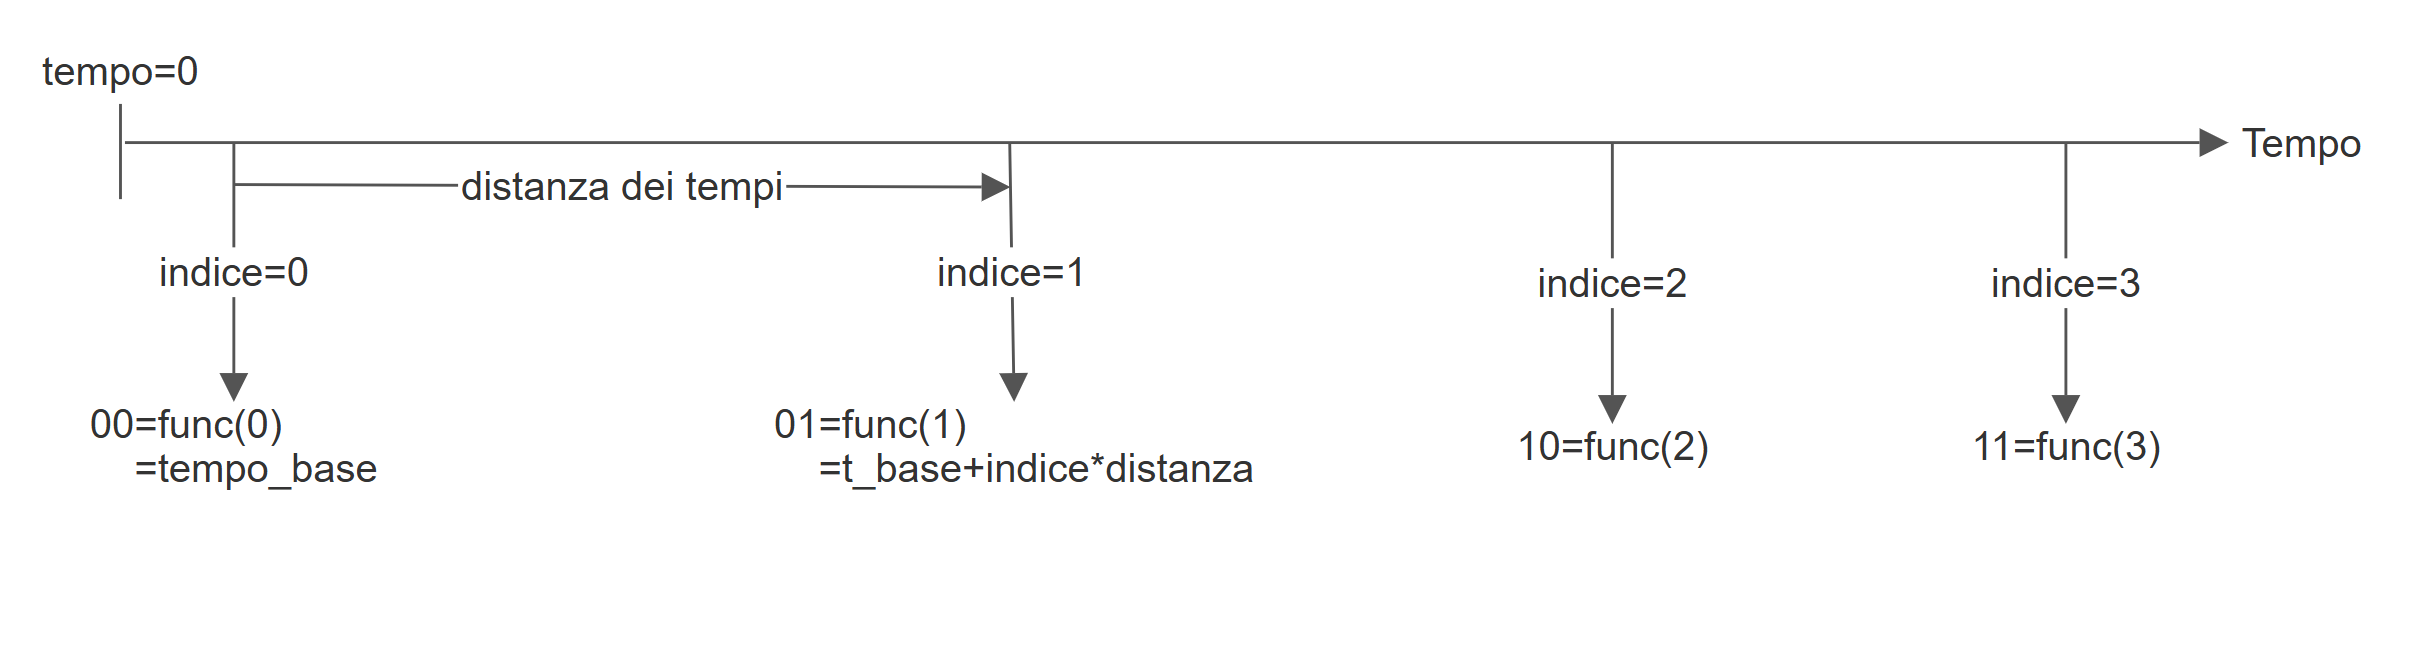
\includegraphics[width=0.9\textwidth]{../Tesi/img/timing_channel/timing_channel_times_nonoverlapping.png}
%    %\captionof{figure}{Assegnazione degli intervalli con la distanza} %di tempo 
%\end{figure} 
%Le distanze fra i vari intervalli di tempo sono 
%necessarie per evitare errori nella decodifica 
%siccome durante la trasmissione del pacchetto possono 
%avvenire dei ritardi sui datagram inviati.
%\end{frame} 

%\begin{frame} 
%\frametitle{Seconda implementazione della funzione}
%Lo svantaggio dell'approccio precedente, sono i tempi 
%di attesa che sono dati dal fatto che il tempo di 
%delay è basato sul valore che lo stesso byte ha. 
%%\vspace{1ex} %\newline
%%Cercando di avere una performance migliore 
%%sui tempi di attesa, si sfrutta il fatto che nella 
%%codifica ASCII i caratteri stampabili vanno da 32 a 
%%126. Si invieranno quindi solo i caratteri stampabili. 
%\begin{columns}[T,onlytextwidth]
%\column{0.48\textwidth}   
%\justifying 
%Quindi si è definita una funzione che normalizzerà 
%l'intervallo di tempo (associato al dato), fra un 
%valore minimo ed uno massimo. Tramite questo approccio, 
%il range dei delay viene ristretto ad un intervallo 
%preciso e definito.  
%\column{0.48\textwidth} 
%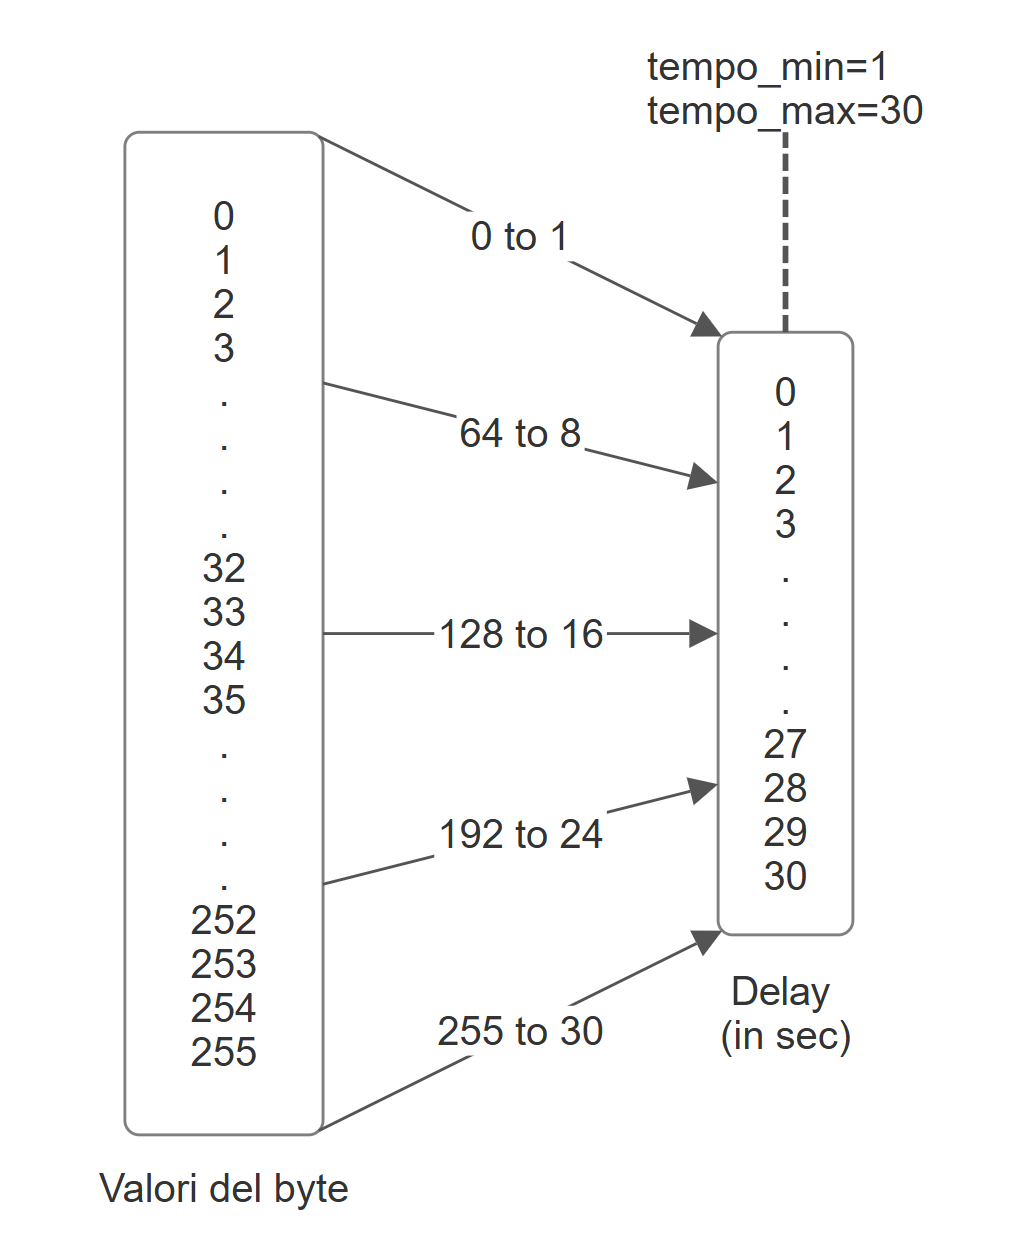
\includegraphics[width=0.65\textwidth]{../Tesi/img/timing_channel/timinmg_channel_2nd_function.png}
%%\captionof{figure}{Normalizzazione degli intervalli (Timing Channel) \cite{time_normalization4}} 
%\end{columns} 
%\vspace{1ex}
%\begin{center}
%    $\text{min\_delay}+(\text{byte}/255)*(\text{max\_delay}-\text{min\_delay})$
%\end{center} 
%\end{frame} 

\begin{frame} 
\frametitle{Implementazione della funzione}
In una prima implementazione si  ricava il tempo di 
delay associando ad ogni valore una distanza temporale 
in base alla distanza che due dati devono avere fra 
di loro. 
\begin{figure}
    \centering 
    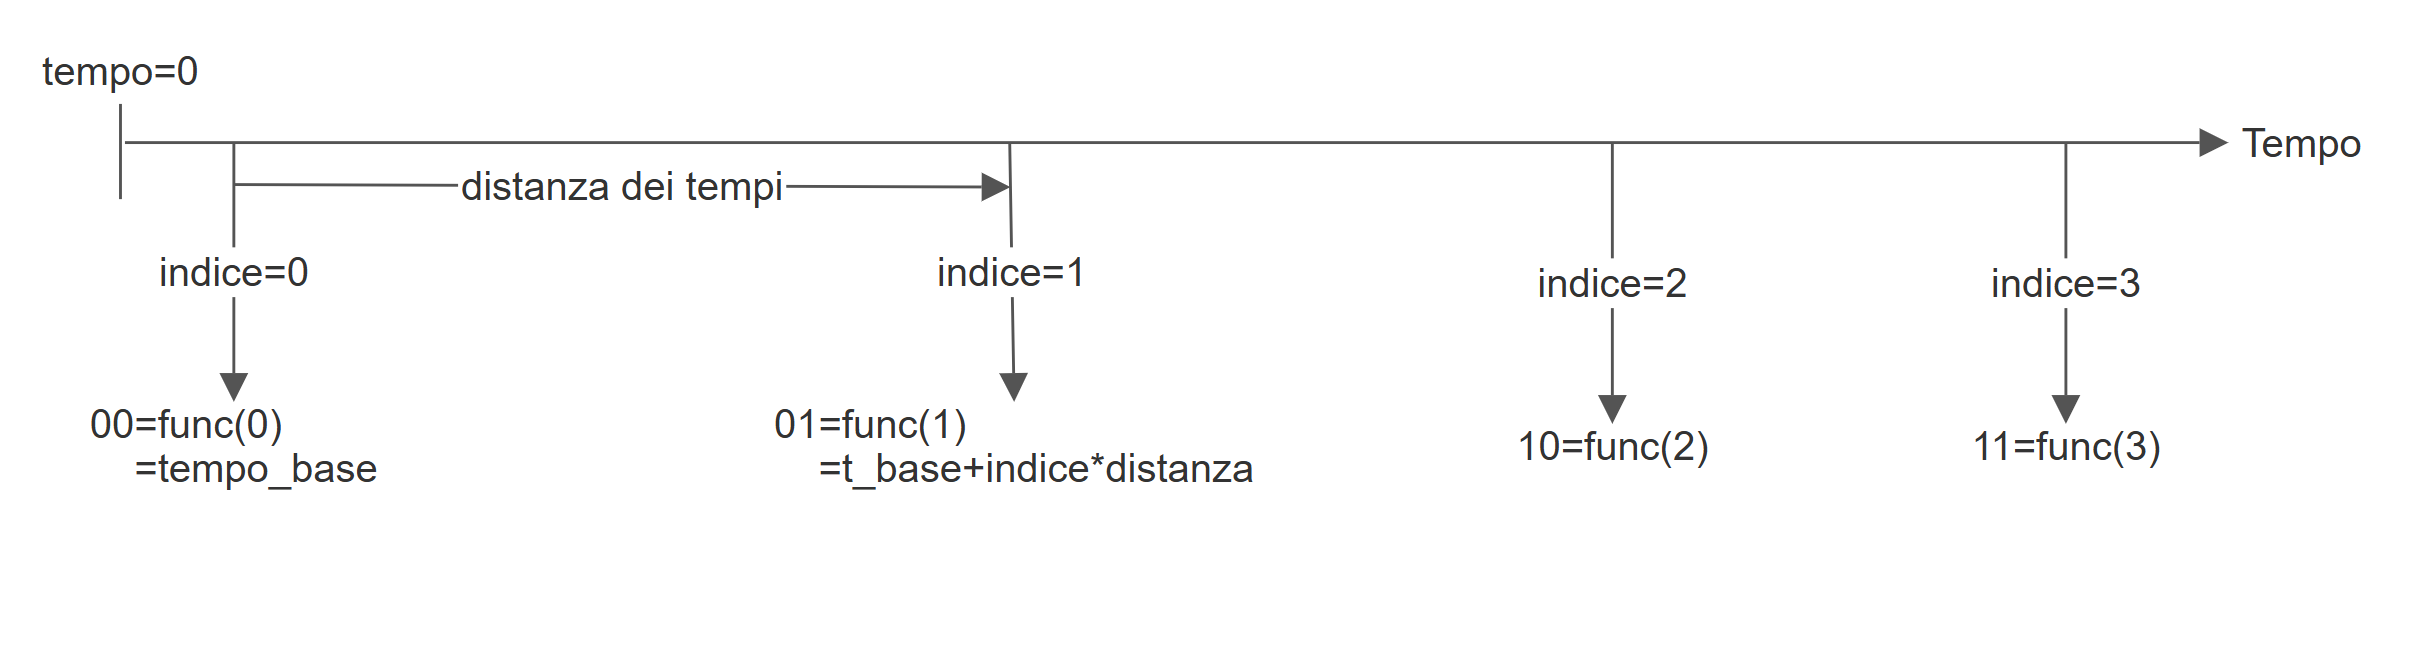
\includegraphics[width=0.8\textwidth]{../Tesi/img/timing_channel/timing_channel_times_nonoverlapping.png}
\end{figure} 
\begin{center}
    $\text{tempo\_base}+\text{indice}*\text{distanza\_tempi}$
\end{center} 
Lo svantaggio dell'approccio sarà relativo ai tempi 
che si aspetteranno. Per risolve il problema, 
si è pensato di ridurre i valori inviabili solo ai 
caratteri stampabili, che nella codifica ASCII vanno 
da 32 a 126. 
\end{frame} 
\begin{frame} 
Sviluppando meglio l'idea e prendendo spundo da 
ICMP Exfill, il tempo di delay ora viene visto come 
il valore intero del byte che si vuole inviare. 
Dopodichè si normalizzerà l'intervallo dei valori 
ottenibili fra un valore minimo ed uno massimo. 
\begin{center} 
$\text{min\_delay}+(\text{byte}/255)*(\text{max\_delay}-\text{min\_delay})$
\end{center} 
\begin{columns}[T,onlytextwidth]
\column{0.48\textwidth}   
\justifying 
Tramite questo approccio, il range dei delay viene 
ristretto in un intervallo definito. Inoltre 
permetterà di regolare la velocità di trasmissione 
delle informazioni ma sacrificando la sensibilità della 
comunicazione ai ritardi di che possono avvenire 
durante il transito dei pacchetti.   
\column{0.48\textwidth} 
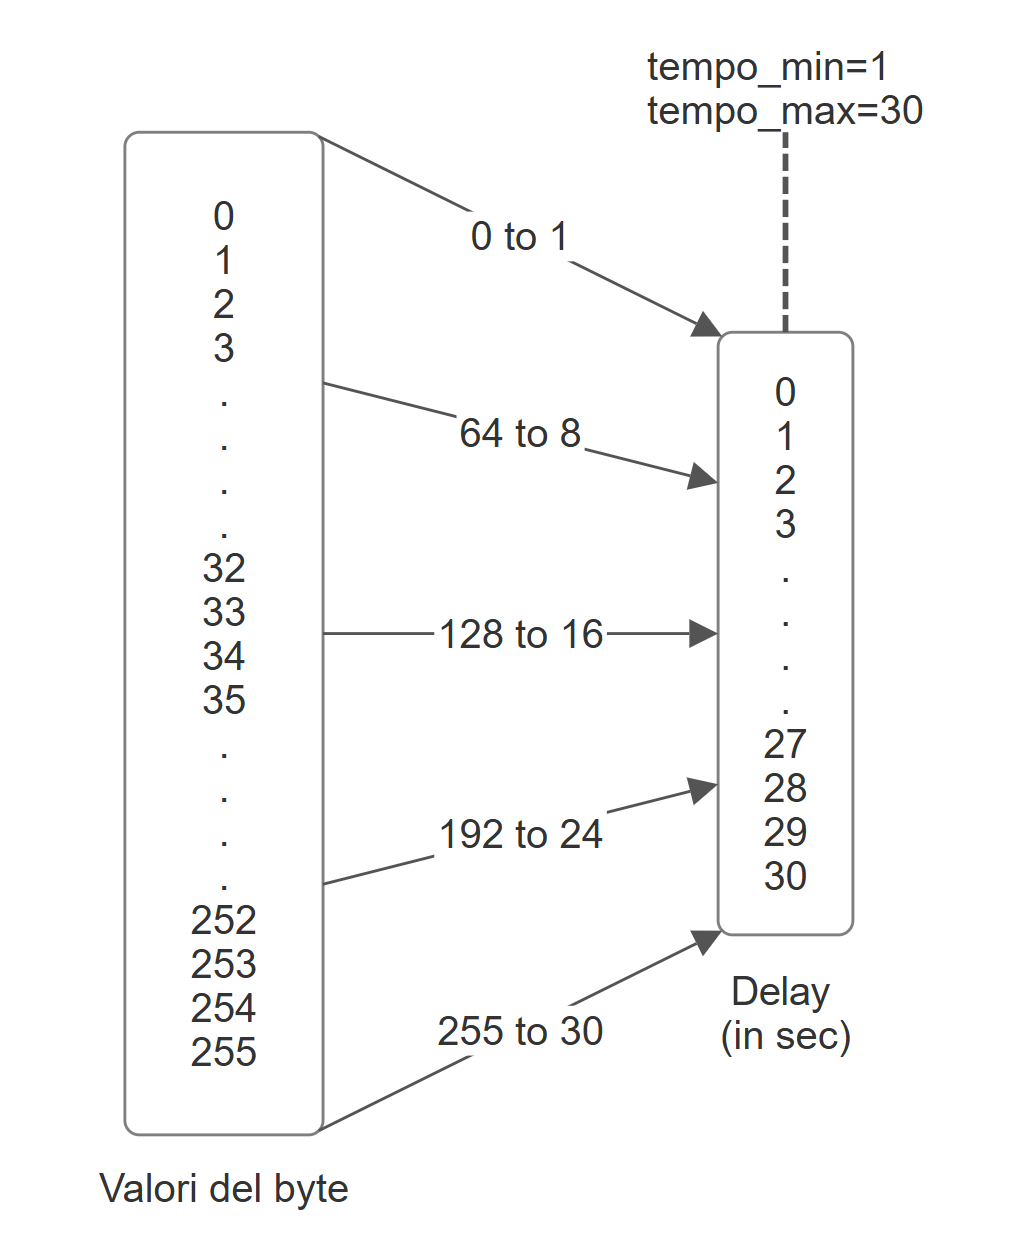
\includegraphics[width=0.7\textwidth]{../Tesi/img/timing_channel/timinmg_channel_2nd_function.png}
\end{columns}  
\end{frame} 
\begin{frame}
%\frametitle{Randomizzazione dei tempi di invio} 
Una funzione in cui lo schema dei tempi di invio dei 
pacchetti sembri casuale, permetterà di essere rilevati 
con maggiore difficoltà. Si agiungerà quindi al Timing 
Covert Channel del rumore così che i tempi di delay 
sembrino casuali. 
\begin{figure} 
    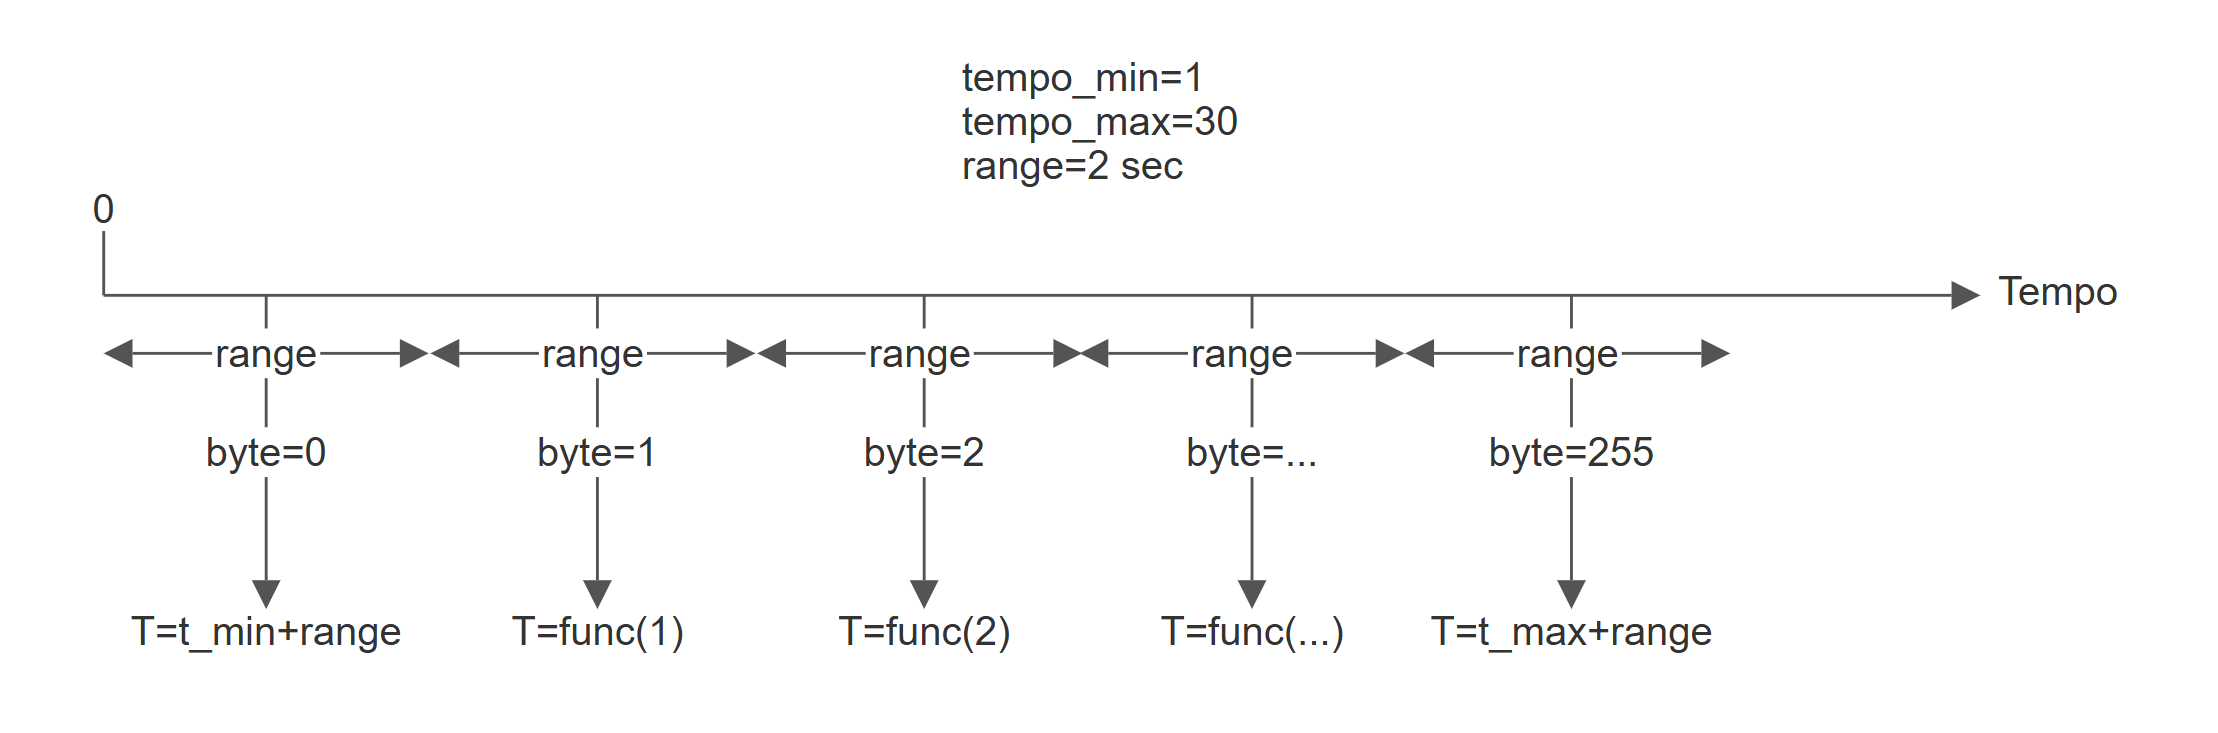
\includegraphics[width=0.8\textwidth]{../Tesi/img/timing_channel/timinmg_channel_rumore.png}
    %\captionof{figure}{Randomizzazione dei tempi con il rumore (Timing Channel)} 
\end{figure}
Ciò porta alla necessita che, per potersi scambiare i dati, il mittente e 
il destinatario devono sincronizzarsi sulla quantità di rumore aggiunto. 
Inoltre al destinatario dovrà essere indicato l'inizio 
della trasmissione o tramite un particolare valore 
o una particolare tipologia di messaggio. 
\end{frame}  
%\begin{frame}
%\frametitle{Requisiti per la comunicazione}
%Siccome il destinatario rimane in ascolto e, all'arrivo di un pacchetto, 
%ricava il dato associato all'intervallo di tempo; avrà bisogno di un 
%messaggio che indichi quando la trasmissione inizia. Nel timing channel si 
%dovrà quindi prevedere un modo per indicare l'inizio della comunicazione. 
%Il metodo potrà essere una particolare sequenza inserita in un campo del 
%pacchetto mentre oppura una particolare tipologia di messaggio ICMP 
%(se non entrambi i metodi). 
%\end{frame}
